\documentclass{article}
\usepackage{graphicx}
\usepackage[margin=1.5cm]{geometry}
\usepackage{amsmath}

\begin{document}
\twocolumn

\title{Thursday Warm Up, Unit 0: Foundations and Fundamentals}
\author{Prof. Jordan C. Hanson}
\maketitle

\section{Memory Bank}
\small
\begin{itemize}
\item \textbf{Homogeneous system:} Let $k$ be a constant, and let $s_{\rm in}(t)$ and $s_{\rm out}(t)$ be the input and output signals to a system $S$, respectively.  $S$ is \textit{homogeneous} if:
\begin{align}
s_{\rm out}(t) &= S[s_{\rm in}(t)] \\
k s_{\rm out}(t) &= S[k s_{\rm in}(t)]
\end{align}
\item \textbf{Additive system:} Let $s_{\rm 1}(t)$ and $s_{\rm 2}(t)$ be two input signals to a system $S$, with outputs $s'_{\rm 1}(t)$ and $s'_{\rm 2}(t)$.  $S$ is \textit{additive} if:
\begin{align}
s'_{\rm 1}(t) &= S[s_{\rm 1}(t)] \\
s'_{\rm 2}(t) &= S[s_{\rm 2}(t)] \\
s'_{\rm 1}(t)+s'_{\rm 2}(t) &= S[s_{\rm 1}(t)+s_{\rm 2}(t)]
\end{align}
\item \textbf{Shift-invariant system:} Let $s_{\rm in}(t)$ and $s_{\rm out}(t)$ be input and output signals to a system $S$, and let $t_0$ be a constant.  $S$ is \textit{shift invariant} if:
\begin{align}
s_{\rm out}(t) &= S[s_{\rm in}(t)] \\
s_{\rm out}(t-t_0) &= S[s_{\rm in}(t-t_0)] \\
\end{align}
\item \textbf{Synthesis:} combining input signal components together linearly to form an output signal.
\item \textbf{Decomposition:} producing the output signal components linearly from an input signal.
\item \textbf{Fundamental Concept of DSP:} Decomposing an input signal into components, passing them trough a linear system, and synthesizing the results produces the same output as passing the original signal through the system.
\item \textbf{Impulse signal:} a single nonzero point in a string of zeros.
\item \textbf{Impulse decomposition:} decomposing a digitized, sampled signal into a linear combination of impulse signals.
\item \textbf{Even/Odd decomposition:} decomposing a digitized, sampled signal into even and odd signal components.
\item $f(-t) = f(t)$ ... Even function.  Even signals: $x_{\rm E}[n] = (x[n] + X[N-n])/2$
\item $f(-t) = -f(t)$ ... Odd function.  Odd signals: $x_{\rm O}[n] = (x[n] - X[N-n])/2$
\end{itemize}
\normalsize

\section{Linear Systems}

\begin{enumerate}
\item Develop an expression for $y_3[n]$ in Fig. \ref{fig:1}.  Which sub-systems must be homogeneous, additive, and shift-invariant, so that $y_3[n]$ retains these properties? \\ \vspace{3cm}
\item Determine if the following functions are even or odd:
\begin{itemize}
\item $\sin(2\pi ft)$:
\item $\exp(-t^2)$:
\item $\exp(-t)$:
\item $at^2 + bt + c$:
\end{itemize} \vspace{1cm}
\item Suppose a system $S$ acts on a signal $x[n]$: $y[n] = S[x[n]]$.  The result is that $x[n]$ is delayed (shifted to the right) by 10 samples, and reduced in amplitude by a factor of 2.  (a) If $x[n] = [0 4 0 0 0 0]$, what is $y[n]$? (b) If $x[n] = [0 0 0 0 2 0]$, what is $y[n]$? \\ \vspace{3cm}
\item (a) Break the signal $x[n] = [0 1 0 0 1 0]$ into component signals that are impulses.  That is, perform an impulse deconposition on $x[n]$. (b) Pass each component through $S$ from the previous exercise, and sum the output signal components.
\end{enumerate}

\begin{figure}
\centering
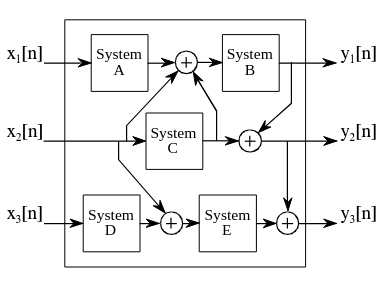
\includegraphics[width=0.33\textwidth]{commute_2.png}
\caption{\label{fig:1} A DSP system with multiple inputs and outputs.}
\end{figure}

\end{document}
